\chapter{Introduction}
\pagenumbering{arabic}

Matter consists of a very large number of interacting particles. In general, we cannot solve their equations of motion exactly $\Rightarrow$ We need to develop numerical methods.\\
If we set out to predict the properties of macroscopic objects from the quantum mechanical description of all their constituents, even numerical methods fail. We cannot handle the time-dependent \textsc{Schrödinger} equation of $10^{23}$ particles, no matter how much of the computer power available today in the world we have access to.\\
Thus, in addition to numerics, we will need statistical mechanics.\\
In this course we will discuss methods to solve statistical mechanics problems on the computer. We begin the course with a brief reminder of the main concepts that lead to the development of statistical mechanics.\\

In the 19\textsuperscript{th} century, the theory of \emph{Thermodynamics} was developed to predict the efficiency of thermal machines, such as the steam engine. Thermodynamics is a macroscopic theory. It deals with large objects and, in particular, time-independent properties (i.e. "equilibrium"). The central notion of Thermodynamics is the fundamental equation, which relates entropy $S$ to internal energy $U$, the particle Number $N$ and the Volume $V$ of an isolated system.

\begin{align}
S &= f(U, V, N)
\end{align}

As $S$ is monotonic in $U$ (this is one of the axioms of Thermodynamics), we can invert $f$ to obtain $U = g(S, V, N)$. The intensive quantities pressure $p$, temperature $T$ and chemical potential $\mu$ are then defined as derivatives of $g$ with respect to $V$, $S$ and $N$.\\
If one knows the fundamental equations for a specific system, one knows its entire equilibrium thermodynamic behaviour, i.e. its reaction to changes in $U$, $V$, $N$ or the conjugate intensive quantities. The latter can be fixed by means of baths ("reservoirs"). To transform the fundamental equation to account for the fixed $T$, $p$ or $\mu$ without loss of information, we simply use a \textsc{Legendre} transformation ($\rightarrow$ therm. potentials).\\
For the entropy of an isolated system there holds an extremization principle, which is carried over to the other thermodynamic potentials.\\

\begin{figure}[!h]
\centering
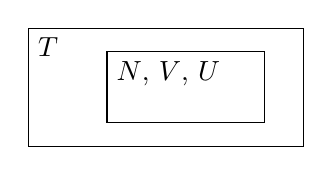
\begin{tikzpicture}
\draw (0,0) node[below right] {$T$} rectangle (3.5,-1.5);
\draw (1, -.3) node[below right] {$N$, $V$, $U$} rectangle (3,-1.2);
\end{tikzpicture}
\caption{A system in contact with a heat bath (and fixed particle number and volume) takes the thermodynamic state which minimizes \emph{free energy}:
$F(N, V, T) = U - TS$}
\end{figure}

We have intuitive notions for $N$ and $V$. And from (quantum) mechanics, we know how to compute energy. But in the 19\textsuperscript{th} century, the microscopic origin of entropy was not clear.\\

Through the works of \textsc{Boltzmann}, \textsc{Gibbs} and others, its relation to the distribution of microstates was discovered:

\begin{figure}[!h]
\centering
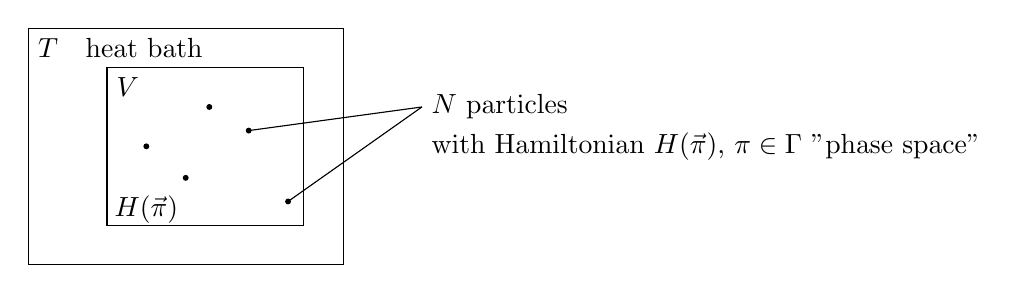
\begin{tikzpicture}
\draw (0, 0) node [below right] {$T$\quad heat bath} rectangle (4, -3);
\draw (1, -.5) node [below right] {$V$} rectangle (3.5, -2.5);
\node at (1.5, -2.3) {$H(\vec{\pi})$};
\filldraw (1.5, -1.5) circle (.03) (2, -1.9) circle (.03) (2.3,-1) circle (.03) (3.3, -2.2) circle (.03) -- (5,-1) node [right] {$N$ particles};
\node[right] at (5, -1.5) {with Hamiltonian $H(\vec{\pi})$, $\pi\in\Gamma$ "phase space"};
\filldraw (5, -1) -- (2.8, -1.3) circle (.03);
\end{tikzpicture}
\caption{TODO}
\end{figure}

probability to find a state $\vec{\pi}$ in $\Gamma$: 
\begin{align}
\rho(\vec{\pi}) = \frac{e^{-\beta H(\vec{\pi})}}{\int e^{-\beta H(\vec{\pi}^\prime)}\ \dd\Gamma^\prime}
\end{align}
